\clearpage
\section{All PSMs of digit recognition}
\label{sec:appendix_digit}
%
% In this section we list the figures that we omitted in the main text.
%
\vspace{2cm}
%
\begin{figure}[htbp]
 \centering
 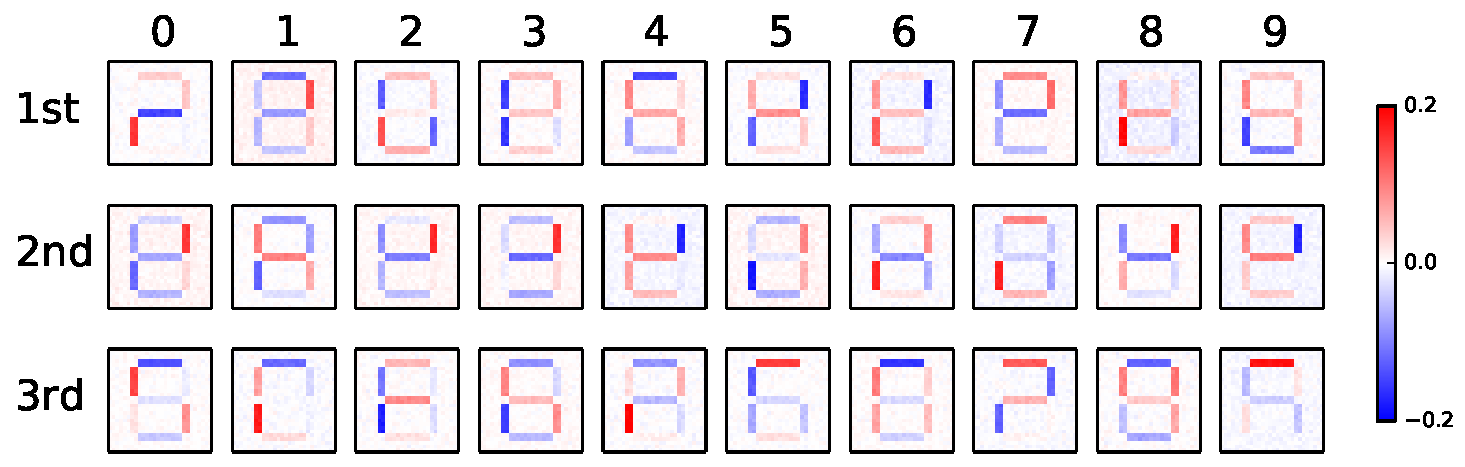
\includegraphics[width=0.9\columnwidth]{./fig/appendix1.pdf}
 \caption{
 First, second and third PSMs of the classifier trained on the artificial dataset.
 }
 \label{app:1}
\end{figure}
%
\vspace{2cm}
%
\begin{figure}[htbp]
 \centering
 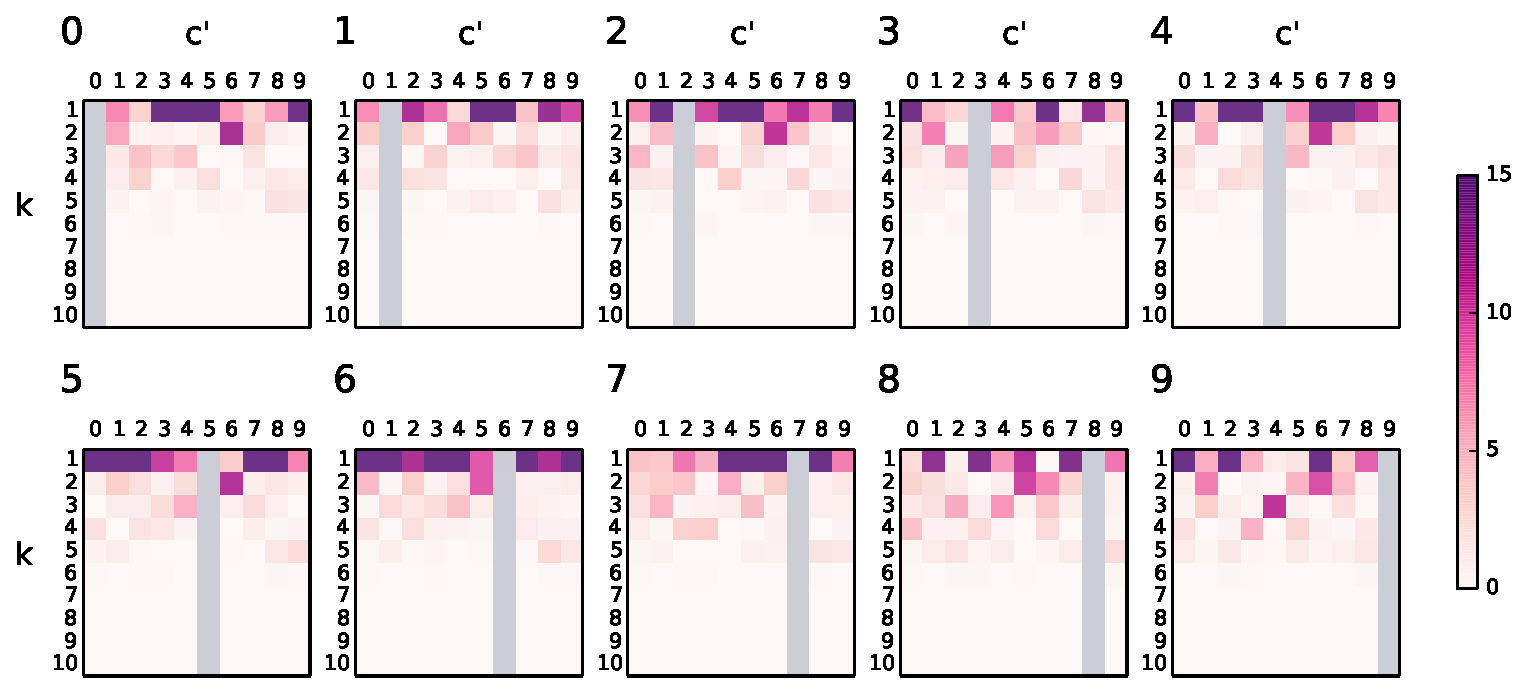
\includegraphics[width=0.9\columnwidth]{./fig/appendix2.pdf}
 \caption{
 $s_{c, c'}(\bvec{v}_{k})$ on the artificial dataset.
 }
 \label{app:2}
\end{figure}
%
\begin{figure}[htbp]
 \centering
 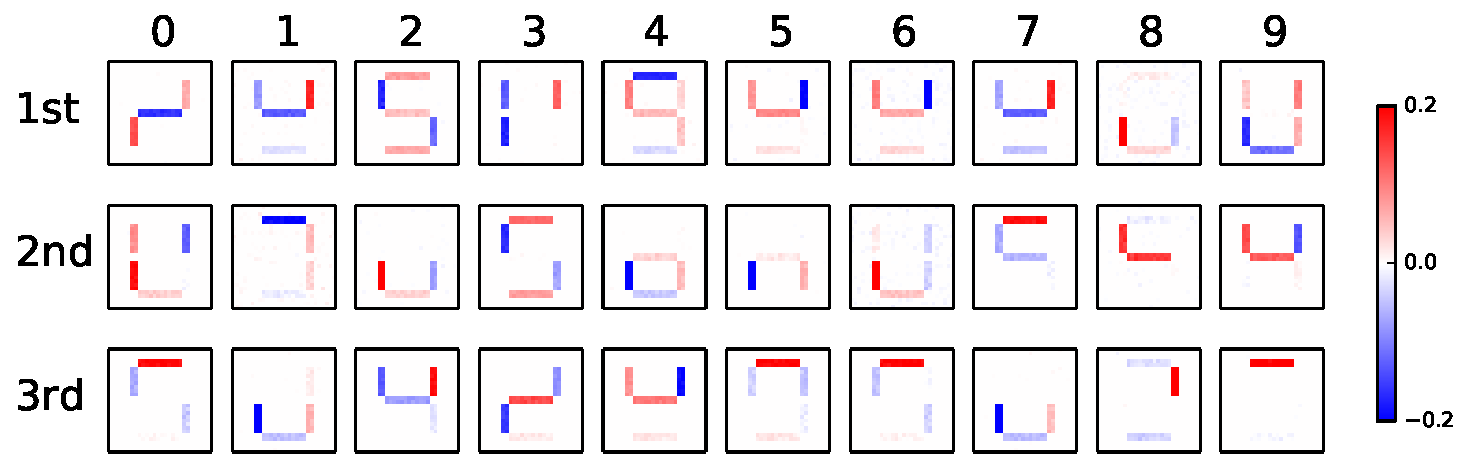
\includegraphics[width=0.9\columnwidth]{./fig/appendix3.pdf}
 \caption{
 Results of the sparse PSA on the classifiers trained on the artificial dataset.
 }
 \label{app:3}
\end{figure}
%
\newpage
\begin{figure}[htbp]
 \centering
 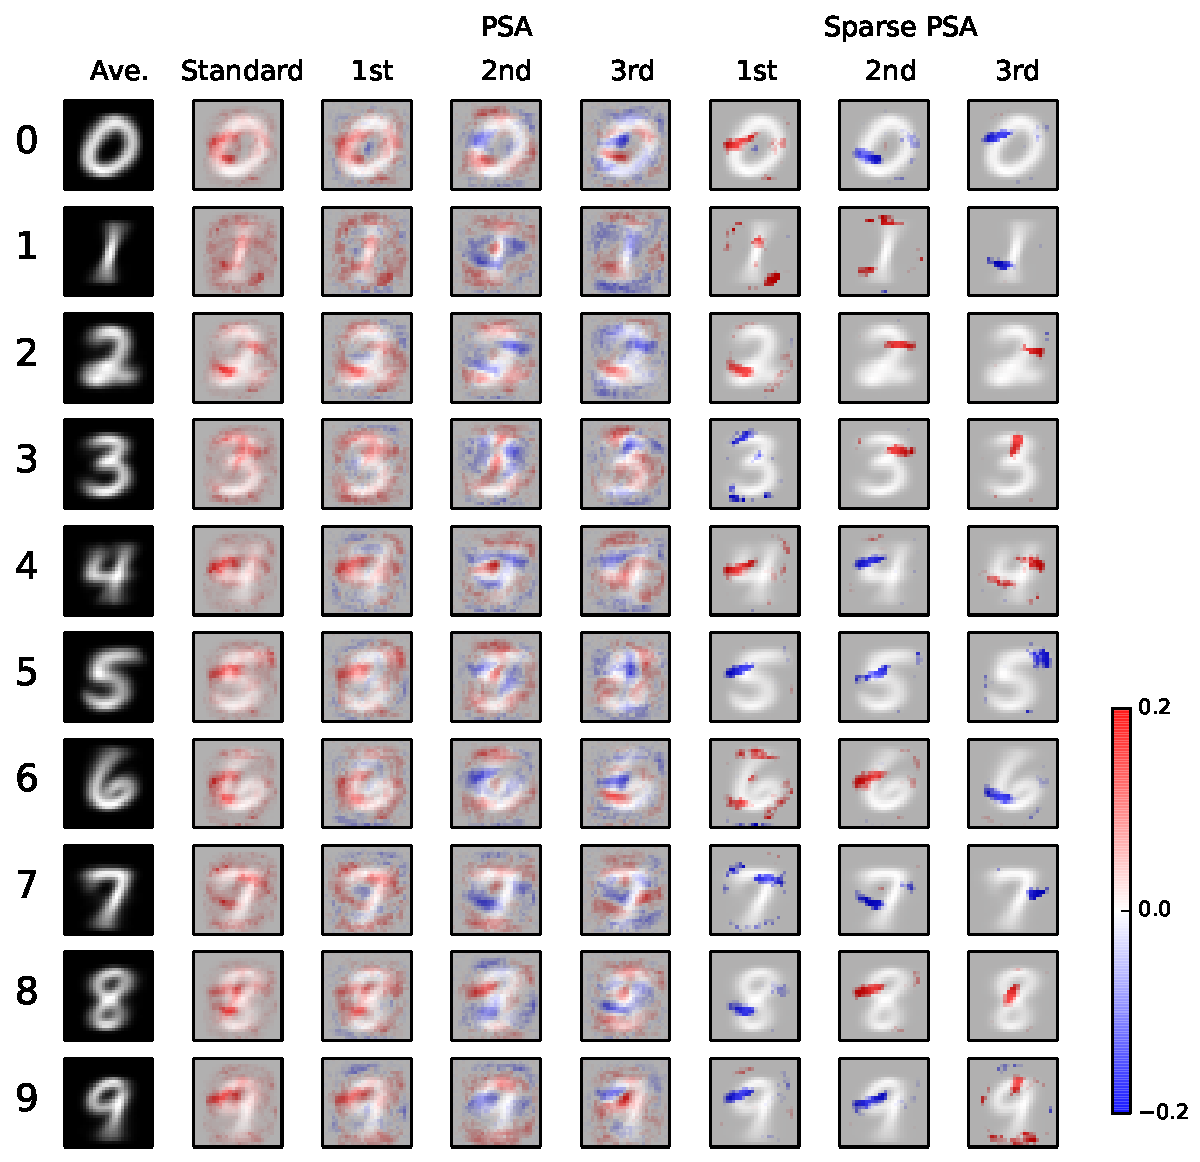
\includegraphics[width=0.9\columnwidth]{./fig/appendix4.pdf}
 \caption{
 Average, standard sensitivity maps, PSMs, and sparse PSMs on MNIST data.
 }
 \label{app:4}
\end{figure}
%
\begin{figure}[htb]
 \centering
 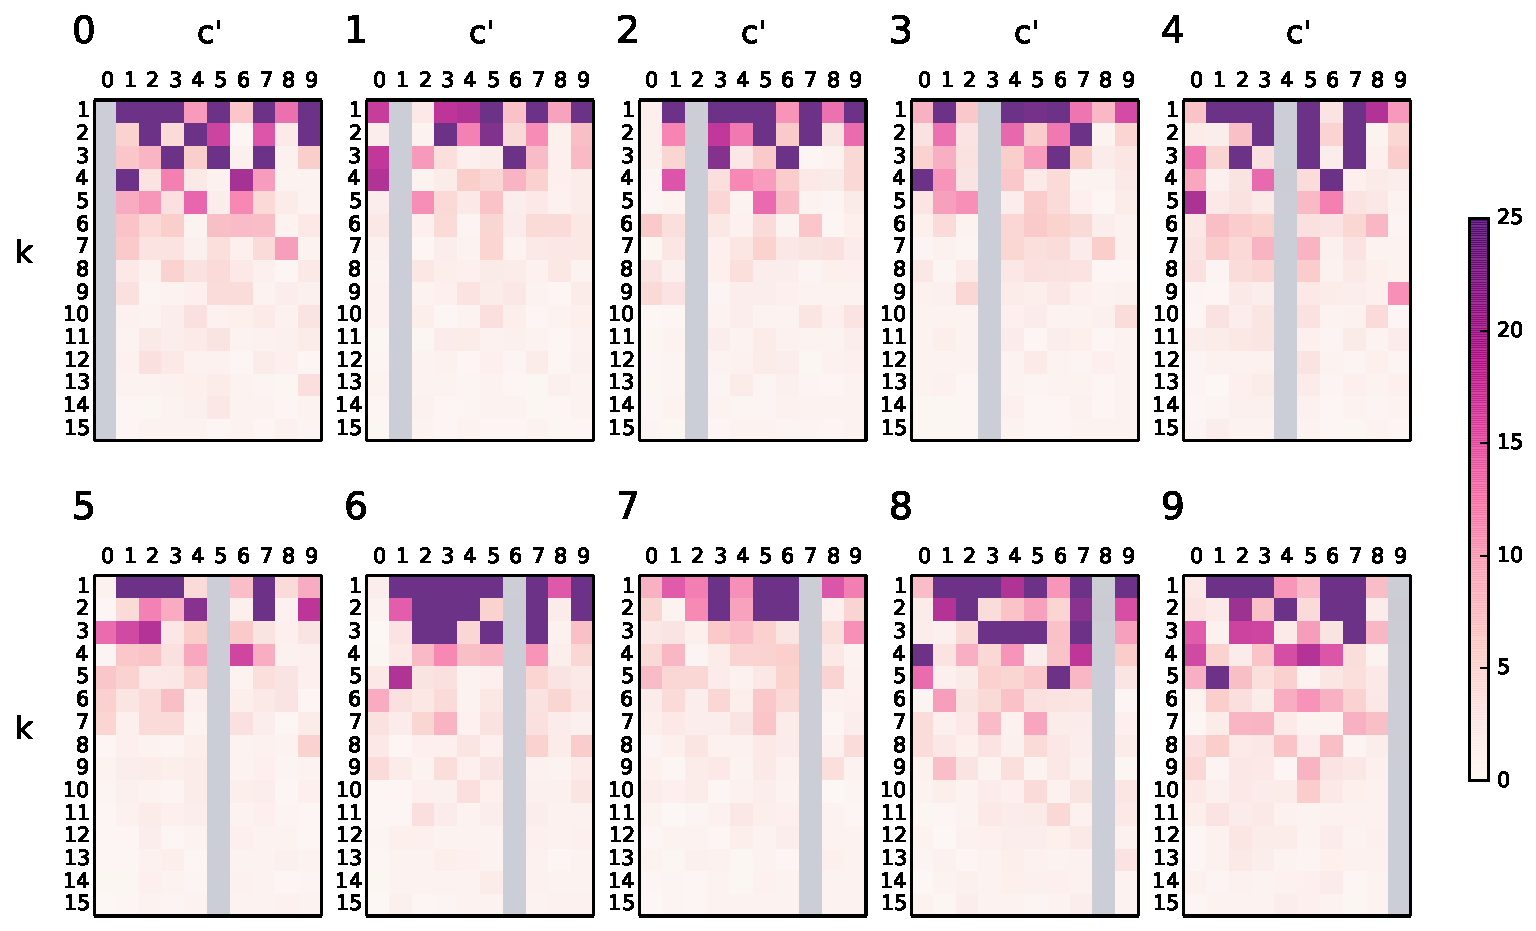
\includegraphics[width=0.9\columnwidth]{./fig/appendix5.pdf}
 \caption{
 $s_{c, c'}(\bvec{v}_{k})$ on MNSIT dataset.
 }
 \label{app:5}
\end{figure}

\clearpage
\section{Specifications of baseline methods}
\label{sec:app_baseline_methods}
%
Each version of SVM consists of seven one-versus-the-rest classifiers.
%
As for the SVMs, we used scikit-learn~\cite{pedregosa2011scikit}.
% hyper parameter
Hyper-parameters were chosen to maximize the decoding accuracy over the validation dataset (see Section~\ref{sec:decoding_setting}); we heuristically prepared nine sets of hyper-parameters for each method, and adopted the one that achieved the best decoding accuracy for the validation dataset.
%
The hyper-parameter for the logistic regression was the learning rate in the MSGD.
%
The hyper-parameter for the linear-kernel SVM was the regularization strength $C$ used in the scikit-learn.
%
The RBM-kernel SVM was dependent on a pair of hyper-parameters, the regularization strength $C$ and the kernel width $\gamma$.
%
We considered $3$ values each for $C$ and $\gamma$, and examined all nine pairs for the best choice.
% END OF PARAGRAPH

\clearpage
\section{All PSMs of subject-transfer decoder}
\label{sec:app_decoding}
%
\begin{figure}[htbp]
\label{fig:appendix_psa}
\begin{center}
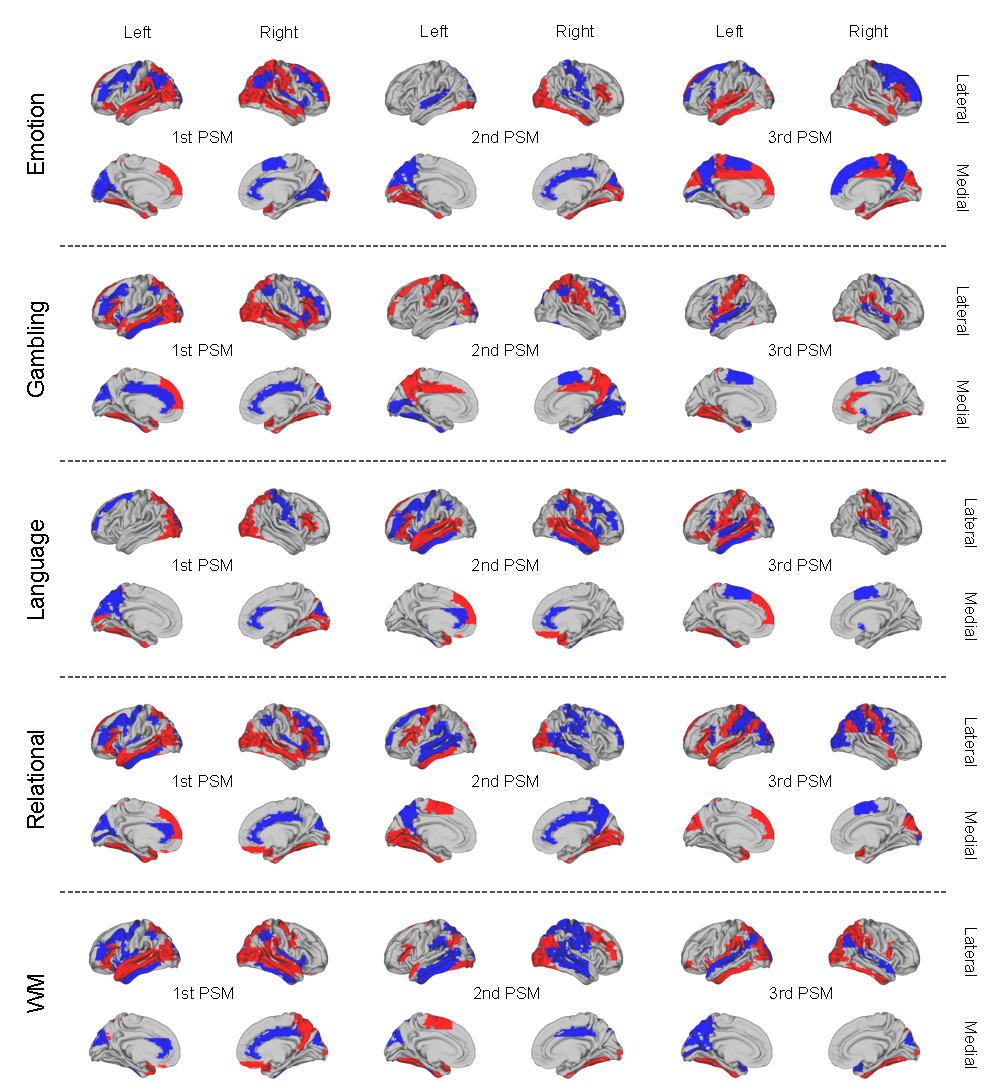
\includegraphics[width=.90\columnwidth]{fig/psa_appendix.pdf}
\caption{PSMs of the other classes (Emotion, Gambling, Language,
 Relational and WM).}
\end{center}
\end{figure}
